\documentclass[12pt, a4paper]{article}
\usepackage{graphicx}
\usepackage[margin=1in]{geometry}
\usepackage{datetime2}
\usepackage[outdir=../images/]{epstopdf} % for adobe scalar graphic
\usepackage{minted} %for clean code
\usepackage{relsize} % for Title
\usepackage{setspace} %remove default header and footer
\usepackage{fancyhdr} %Header
\usepackage{hyperref} % Display Links/ URLs better 
\usepackage{tocloft} % add dots in TOC

\hypersetup{
	linktoc=all,
	colorlinks=true,
	linkcolor=black,
	linktocpage}

% Change the size of the "Contents" title
\renewcommand{\contentsname}{\huge\bfseries Contents} 
\renewcommand{\cftsecleader}{\cftdotfill{\cftdotsep}} % add the dots in Table of Content

\DTMsetstyle{mmddyyyy} %datetime2
\setminted[python]{style=colorful} %set the whole doc for python code.
\fancyhf{}

\begin{document}

\thispagestyle{empty}


\includegraphics[scale=2]{../images/ECS.eps}

\vspace{2in}
\font\tmpfont=cmr12 at 40pt  %useful for large titles
{\centering\tmpfont GitHub x Python Workshop \par}

\vskip30pt

\doublespacing
{\centering\Huge Introduction to Git and GitHub \par}

\vspace{3in}

\begin{flushright}	
	{\Large Hosted by IEEE CSUN\\
	Student Branch}
\end{flushright}
\singlespacing
\newpage

\doublespacing % TOC is in double spacing
\tableofcontents
\addtocontents{toc}{~\hfill\textbf{Page}\par}
\singlespacing % revert back
\newpage

%created the header
\setlength{\headheight}{40pt}
\pagestyle{fancy}
\fancyhead[L]{
\includegraphics[scale=1]{../images/ECS.eps}}
\fancyhead[R]{IEEE CSUN\\GitHub Workshop}
\fancyfoot[R]{Page $|$ \thepage}

\def\tilda{\raisebox{-0.5ex}{\textasciitilde}}

\section{Introduction}
Git is a distributed version control system that helps developers track changes in code, collaborate, and manage projects. This guide will cover all the basics of utilizing git. GitHub is a web platform that uses Git for version control and adds collaboration features. This guide will cover how GitHub is used to back up but also use it as a collaboration platform.
\section{Setup}
We need to first install a Git-bash:\\

\begin{itemize}
    \item Windows: \url{https://gitforwindows.org/}
	\begin{itemize}
		\item Click on Download and download Git-2.XX.x.x-64-bit.exe or Git-2.XX.x.x-arm54.exe
		\end{itemize}

    \item Mac: Install GitHub from the App Store or using Homebrew:
\verb+brew install git+\\
\item Linux:
    \begin{itemize}
        \item If Debian-based: \verb+sudo apt-get install git+ \\
        \item If Fedora-based: \verb+sudo dnf install git+\\
        \item If Arch-based: \verb+sudo pacman -S git+ 
    \end{itemize}
\end{itemize}

\section{Verifying git Installation}

Each Operating system has its own method to running its git client. 
\begin{itemize}
\item Windows: Press the windows key and search up \textbf{Git Bash} and open the Git Bash application.
\item Mac: Open up the terminal using: \texttt{CMD+Space} type in \texttt{Terminal}
\item Linux: Open up the terminal using \texttt{Ctrl+Alt+T}.
\end{itemize}

In the terminal run \verb+git --version+ to verify the installation of git.
\begin{figure}[H]
\centering
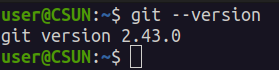
\includegraphics[scale=0.75]{../images/workshop-I/git-ver.png}
\caption{Printing git version}
\end{figure}
\section{Basic Bash (Optional)}
Bash is a programming language that can be used like python. Like how python commands can run on Python's interactive shell, Bash commands can also run in a shell. It runs in the (B)ourne (a)gain (sh)ell usually in your terminal. For many Linux distro's Bash is the default and for Mac its Zsh. For Windows it is Powershell. So in this workshop you will be learning a bit of Linux. Here is some list of basic commands:


\begin{itemize}
    \item \verb`cd`: short for change directory. Used to traversal through the directories in your system. Directories are just folders. Examples:
        \begin{itemize}
		\item \texttt{cd \tilda} or just \verb`cd` :This takes you back to your home directory. Each user on the PC has their own home directory.
		\item \texttt{cd \tilda/Downloads/} :This will take you to your Downloads folder.
            \item \verb`cd ..` :This command take you back a single directory.
            \item \verb`cd ../..` :Takes you back two directories. You can add on to this to go back more directories.
            \item \verb`cd /`  :Take you to the home directory of the system. Usually users can't write any files here.
        \end{itemize}
    \item \verb`ls`: Lists files and directories inside of your current directory. Examples:
        \begin{itemize}
            \item \verb` ls -a`: Lists all files and folders including hidden ones.
    	    \item \texttt{ls \tilda/Downloads/} :It would print out everything in your downloads.
	    \item \texttt{ls -l \tilda/Downloads/} :It would print everything in a list format, all entries in a single format.
        \end{itemize}
    \item \verb`pwd`: short for print working directory. Typing just that print where you are right now.
    \item \verb`cat`: concatenates/prints the file you gave it. Ex. \verb`cat some_file.txt`: It would print out all that's in the file.
    \item \verb`man`: Really useful to read manuals about a command. Ex. \texttt{man ls} tells you everything about the \texttt{ls} command.
    \item \verb`ssh`: This command will allow us to remote access a server.
\end{itemize}

\section{Configuring git}

From now on all the steps for every operating system should be the same.
Git requires its users to confirm people's identity to see who wrote the code. In the terminal type in
\begin{itemize}
\item\verb+git config --global user.email "your_email_address_here”+
\end{itemize}
Following that set up your username:
\begin{itemize}
\item \verb+git config --global user.name "your_user_name_here"+
\end{itemize}

Typing \texttt{git config --list} or \texttt{cat \tilda/.gitconfig} can help you verify if you set it up properly.\\\par
\textbf{Note:} Use your GitHub email and username to have a seamless transition when working with GitHub.

\begin{figure}[H]
\centering
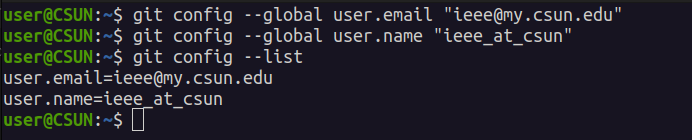
\includegraphics[scale=0.5]{../images/workshop-I/git-config.png}
\caption{Configuring Git}
\end{figure}
\section{Creating a Repository}

After all this info dump of setting up git. Here is where we can get started. Log in to your GitHub account. Then, on the home page, click the \textbf{New} button. Give the repo the name \textbf{Python-RPS} and add a README file.
\begin{figure}[H]
\centering

\includegraphics[scale=0.5]{../images/workshop-I/GH-new-repo.png}
\caption{New repo button}
\end{figure}
\begin{figure}[H]
\centering
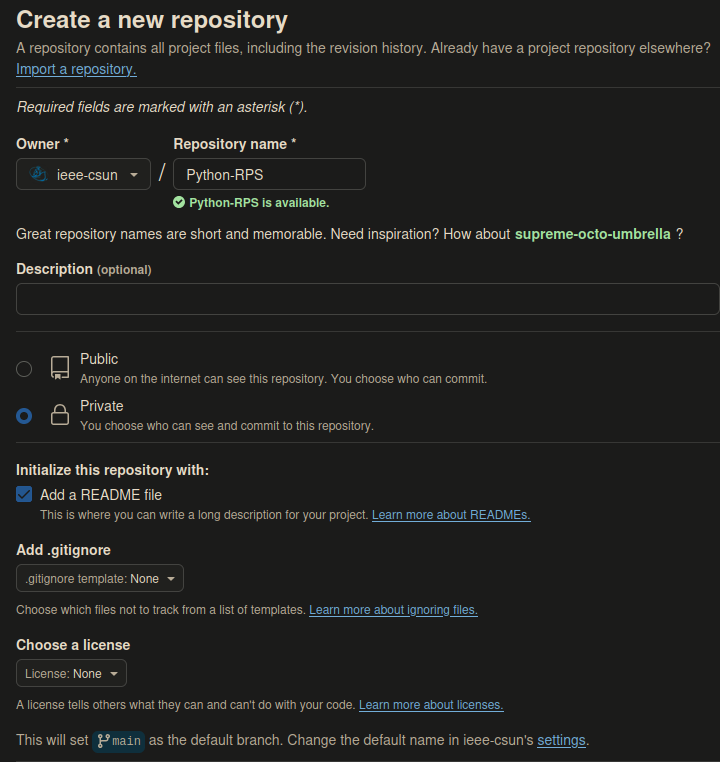
\includegraphics[scale=0.5]{../images/workshop-I/GH-create-repo.png}
\caption{Creating the Repo}
\end{figure}
\section{Setting up Authentication}

Now that you created the repository, you need a way to let GitHub know that the person accessing your repository is you. This is done by using private and public key pairs. \\\\
In the terminal enter the follow command:\\
\texttt{ssh-keygen -t ed25519 -C "your\_github\_email\_here”}\\

\noindent There will be a prompt asking you to choose where to save the key pair, leave it at its default location by pressing \textbf{Enter.} A second prompt will ask to create a password to further encrypt the key pair, you can press enter to not add a password if you choose so.\\\\
\textbf{Note:} Having a password will ask you to enter the password every time you boot up your PC. \\

\begin{figure}[H]
\centering
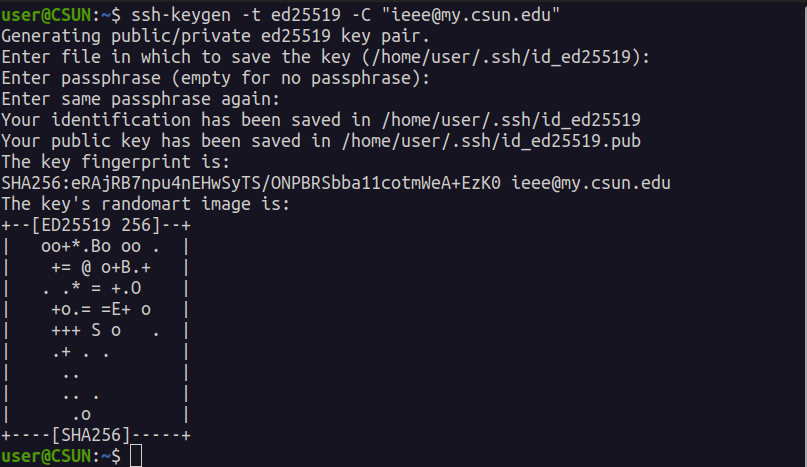
\includegraphics[scale=0.4]{../images/workshop-I/key-gen.png}
\caption{SSH key generating}
\end{figure}

\noindent\textbf{For Windows Users}: Enter following to start you ssh-agent: \texttt{eval "\$(ssh-agent -s)”} Now read the following steps like everyone else.\\

\noindent \textbf{All Users:} Add your private key to the ssh-agent using this command:\\
\texttt{ssh-add \tilda/.ssh/id\_ed25519} Next step is to copy the public ssh key to GitHub. Firstly run \texttt{cat \tilda/.ssh/id\_ed25519}\textbf{.pub} to print out the key and then head over to \url{https://github.com/settings/keys} or do it manually by clicking on the user profile then ``Settings" then to ``SSH and GPG keys"and add a new SSH key. To verify you have done all these steps correctly run \texttt{ssh -T git@github.com} 
\begin{figure}[H]
\centering
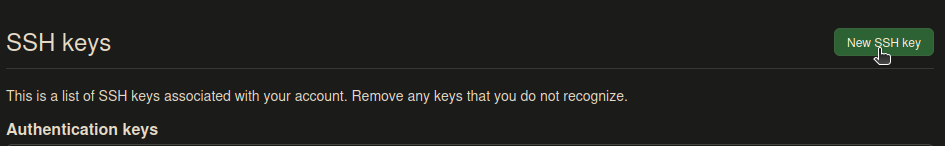
\includegraphics[scale=0.4]{../images/workshop-I/GH-new-key.png}
\caption{Creating a new key to GitHub}
\end{figure}
\begin{figure}[H]
\centering
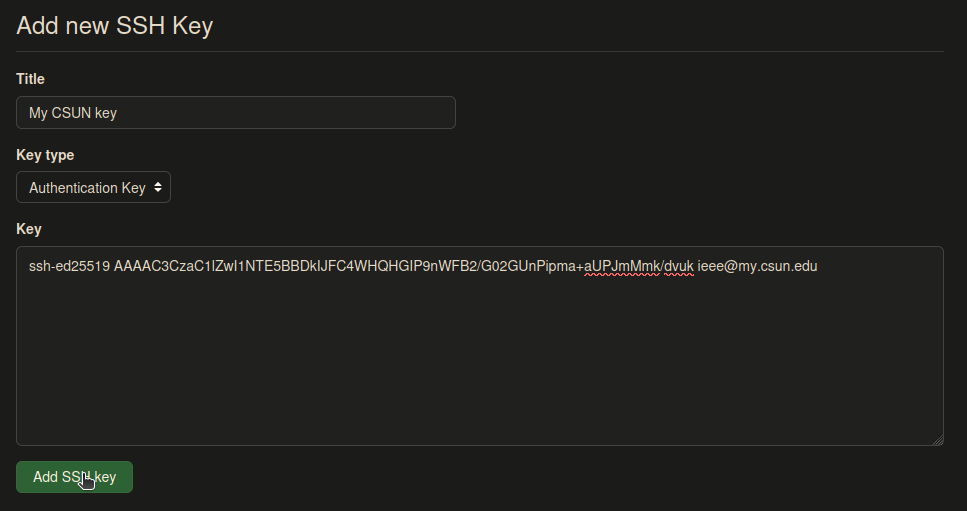
\includegraphics[scale=0.5]{../images/workshop-I/GH-add-key.png}
\caption{Adding Key to GitHub}
\end{figure}
\begin{figure}[H]
\centering
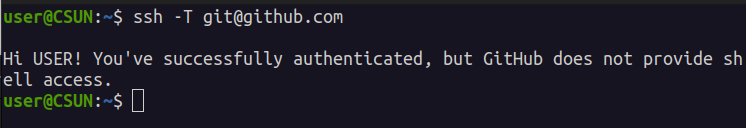
\includegraphics[scale=0.5]{../images/workshop-I/ssh-T.png}
\caption{SSH output when logging into GitHub.}
\end{figure}

\section{Cloning a Repository}

Head over to your GitHub Repository that you have created for this Python Project. There you will find a green button labeled ``Code". Click this button and select the SSH key menu. Here you can copy the SSH key for your GitHub repo. \\

Syntax: \texttt{git clone URL\_HERE}\\

\noindent \textbf{Make sure} to \texttt{cd Python-RPS/}. Using the above you can clone the GitHub repo into your personal system. From here it is simply a matter of opening your programming IDE and creating a python file in the created directory.
\begin{figure}[H]
\centering
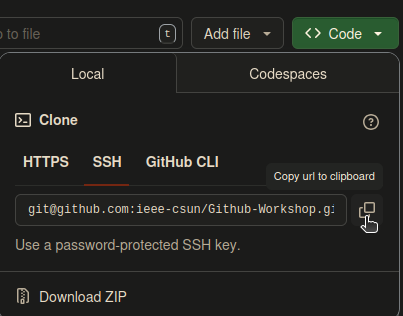
\includegraphics[scale=0.5]{../images/workshop-I/GH-URL.png}
\caption{Copying the URL}
\end{figure}
\begin{figure}[H]
\centering
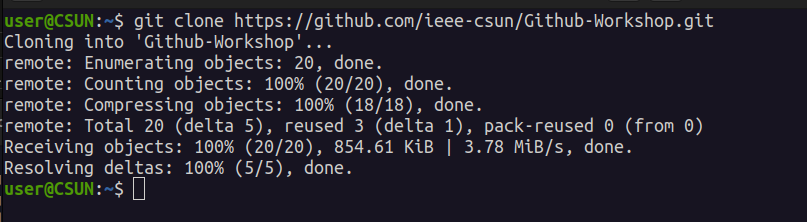
\includegraphics[scale=0.5]{../images/workshop-I/git-clone.png}
\caption{Cloning a repo}
\end{figure}


\section{Adding Local Repository (Optional)}
Because of GitHub's capability of backing up your repo and encouraging collaboration between others. Commands to run:
\begin{itemize}
    \item \verb`git init` will change the directory you are on to a git repo. you can check by doing \verb`ls -a` and look for a .git folder.
    \item Head over to GitHub to create a new \textbf{empty} repo. You will be syncing your local git repo to that remote repo.
    \item \verb`git remote add origin <URL>` this will add the URL to your local repo. For us, use \verb`git@github.com:USERNAME/REPO.git` because we setup ssh verification.
    \item Now make sure to \verb`git add -A` your files and make a commit.
    \item Last step is to push the changes we do that by running. \verb`git push -u origin main`
\end{itemize}

\section{Storing Changes}

When you have a git repo you are bound to make changes that you want to save and log so that you can revert changes later if something goes wrong. How do you save snapshots of your code? In git, we use \texttt{git commit}. To start off we run the command \texttt{git status -u} to see if there are any changes that need to be saved. If there are unsaved changes we add the files to a staging area where the files are waiting to be commited. We do that by either using \texttt{git add <file\_name>} or \texttt{git add -A} to commit all files. To commit our changes we do \texttt{git commit -m "a message about what you did"}. Final step is to store those changed made to the cloud, in our case to Github. We do that by running \texttt{git push} where we push the changes.\\

\textbf{Note:} In the future on you run \texttt{git add -u} to add just the updated files. Doing \texttt{git add -A} may add unwanted files. To avoid such scenario from ever happening we create a file called \verb+.gitignore+ where we can enter the file type, location, file name or all three combined should be ignored.
\begin{figure}[H]
\centering
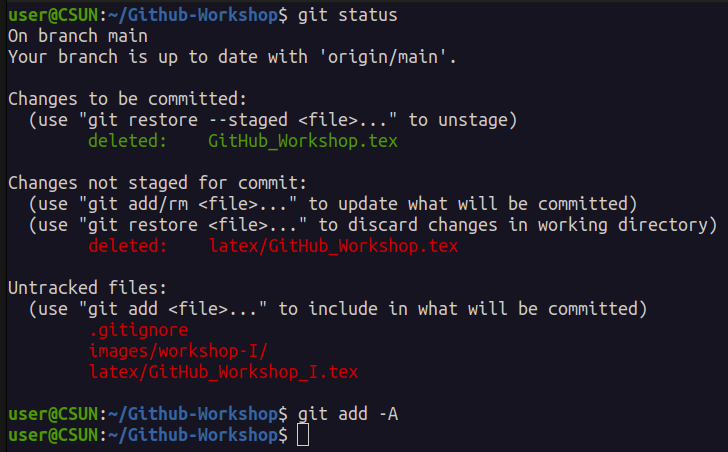
\includegraphics[scale=0.5]{../images/workshop-I/git-add.png}
\caption{Git status simple with git add all}
\end{figure}
\begin{figure}[H]
\centering
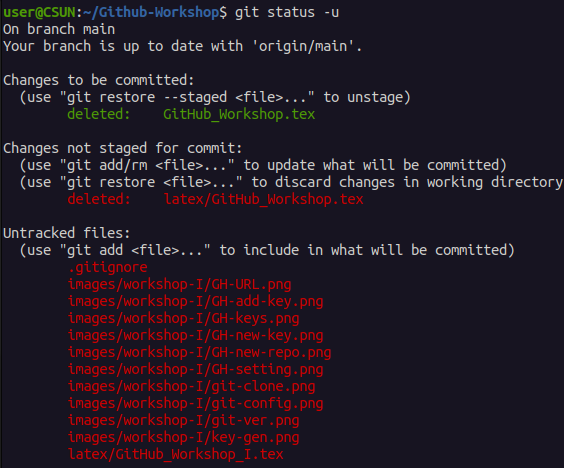
\includegraphics[scale=0.5]{../images/workshop-I/git-status-u.png}
\caption{Git status detailed}
\end{figure}

\begin{figure}[H]
\centering
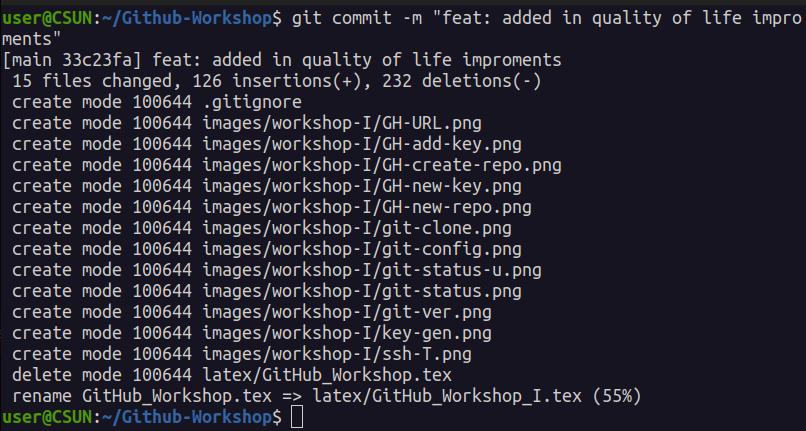
\includegraphics[scale=0.5]{../images/workshop-I/git-commit.png}
\caption{Git commit example}
\end{figure}

\begin{figure}[H]
\centering
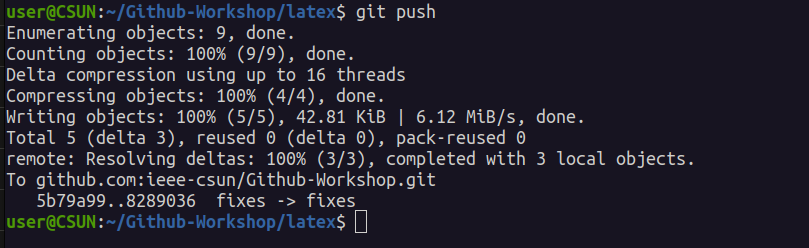
\includegraphics[scale=0.5]{../images/workshop-I/git-push.png}
\caption{Git push example}
\end{figure}

\section{Frequently Used Commands}
\begin{itemize}
    \item \verb`git pull`: Always to this when you start working of the project if you are collaborating.
    \item \verb`git status`: This is to know what files are tracked and which files are not.
    \item \verb`git add file_name` and \verb`git reset file_name`: When you want to stage or unstage files from the project. While \verb`git rm` deletes the file \textbf{permanently}.
    \item \verb`git commit -m "message"`: To backup changes to the code.
    \item \verb`git push`: When you want to upload files to GitHub.
\end{itemize}
For more resources: \url{https://education.github.com/git-cheat-sheet-education.pdf}
\clearpage

\section{Python Task}
The following code is what you will be working to do today. You can download the code from the Latex Workshop GitHub page.
\begin{minted}[breaklines]{python}
import random

# Print game rules
print('Winning rules of the game ROCK PAPER SCISSORS are:\n'
      + "Rock vs Paper -> Paper wins \n"
      + "Rock vs Scissors -> Rock wins \n"
      + "Paper vs Scissors -> Scissors wins \n")

while True:
    print("Enter your choice \n 1 - Rock \n 2 - Paper \n 3 - Scissors \n")

    # TODO: Get and convert user input
    # HINT: Use input() to read from the user and wrap it with int()
    choice = ___

    # TODO: Keep asking until the input is valid (between 1 and 3)
    # HINT: Use a while loop to check if choice is not in the valid range
    while ___:
        choice = ___

    # TODO: Map the user’s choice to its name
    # HINT: Use if-elif-else to assign choice_name based on choice number
    if choice == ___:
        choice_name = '___'  # HINT: This should be "Rock"
    elif ___:
        choice_name = '___'  # HINT: This should be "Paper"
    else:
        choice_name = '___'  # HINT: This should be "Scissors"

    print('User choice is:', choice_name)
    print("Now it's Computer's Turn...")

    # TODO: Computer makes a random choice
    # HINT: Use random.randint() with range 1 to 3
    comp_choice = ___

    # TODO: Map computer's choice to its name
    if ___:
        comp_choice_name = '___'
    elif ___:
        comp_choice_name = '___'
    else:
        comp_choice_name = '___'

    print("Computer choice is:", comp_choice_name)
    print(choice_name, 'vs', comp_choice_name)

    # TODO: Determine the winner
    # HINT: First handle tie, then combinations where Paper, Rock, or Scissors win
    if ___:
        result = "DRAW"
    elif (choice == ___ and comp_choice == ___) or (choice == ___ and comp_choice == ___):
        result = '___'  # HINT: Paper wins in this case
    elif (___ and ___) or (___ and ___):
        result = '___'  # HINT: Rock wins in this case
    elif (___ and ___) or (___ and ___):
        result = '___'  # HINT: Scissors wins in this case

    # TODO: Print game result
    # HINT: Compare result with "DRAW" and with user choice_name
    if ___:
        print("<== It's a tie! ==>")
    elif ___:
        print("<== User wins! ==>")
    else:
        print("<== Computer wins! ==>")

    # TODO: Ask to play again
    # HINT: Use input() and convert to lowercase
    print("Do you want to play again? (Y/N)")
    ans = ___.___()
    if ans == 'n':
        break

print("Thanks for playing!")

\end{minted}

\end{document}
